\documentclass[10pt,letterpaper]{article}
\usepackage[latin1]{inputenc}
\usepackage{amsmath}
\usepackage{amsfonts}
\usepackage{amssymb}
\usepackage{graphicx}
\usepackage{framed}
\usepackage{pdfpages}

\author{Jonas Kersulis}
\title{Lagrange multiplier proof}

\begin{document}
\maketitle
%
%\textbf{Problem}
%\begin{align*}
%&(P) &\min~ & z^\top C z - 2b^\top z & \\
%& s.t. & z^\top z &= s^2
%\end{align*}
%
%\textbf{Claim [Gander 1989]}: $(P)$ is equivalent to
%\begin{align*}
%&(P') & \min~ & \lambda  \\
%& s.t.& z^\top z &= s^2 \\
%&& Cz &= \lambda z + b
%\end{align*}
%In general, there are many solutions $\lambda$ to the first-order conditions
%\begin{subequations}\label{eq:first}
%\begin{align}
%\label{eq:first1}Cz &= \lambda z + b \\
%\label{eq:first2}z^\top z &= s^2
%\end{align}
%\end{subequations}
%Gander's claim is that the objective of $(P)$ is minimized when the \textit{smallest} value of $\lambda$ is chosen. The following proof formalizes this claim.
%
%\textbf{Theorem:} if $(\lambda_1,z_1)$ and $(\lambda_2,z_2)$ solve \eqref{eq:first}, and $\lambda_1 < \lambda_2$, then
%\begin{align*}
%z_1^\top C z_1 - 2b^\top z_1 &< z_2^\top C z_2 - 2b^\top z_2
%\end{align*}
%\textbf{Proof:} Multiply \eqref{eq:first1} by $z_1^\top$ and $z_2^\top$ for both $z_1$ and $z_2$:
%\begin{subequations}
%\begin{align}
%\label{eq:2a}z_1^\top C z_1 &= \lambda_1z_1^\top z_1 + z_1^\top b = \lambda_1 s^2 + z_1^\top b \\
%\label{eq:2b}z_2^\top C z_2 &= \lambda_2z_2^\top z_2 + z_2^\top b = \lambda_2 s^2 + z_2^\top b \\
%\label{eq:2c}z_1^\top C z_2 &= \lambda_2z_1^\top z_2 + z_1^\top b \\
%\label{eq:2d}z_2^\top C z_1 &= \lambda_1z_2^\top z_1 + z_2^\top b
%\end{align}
%\end{subequations}
%Subtract \eqref{eq:2b} from \eqref{eq:2a}:
%\begin{align*}
%(z_1^\top C z_1 - z_1^\top b) - (z_2^\top C z_2 - z_2^\top b) &= (\lambda_1 - \lambda_2)s^2
%\end{align*}
%Add $z_2^\top b$ and subtract $z_1^\top b$:
%\begin{align*}
%(z_1^\top C z_1 - 2z_1^\top b) - (z_2^\top C z_2 - 2z_2^\top b) &= (\lambda_1 - \lambda_2)s^2 - z_1^\top b + z_2^\top b
%\end{align*}
%Substitute \eqref{eq:2c} and \eqref{eq:2d}:
%\begin{align*}
%(z_1^\top C z_1 - 2z_1^\top b) - (z_2^\top C z_2 - 2z_2^\top b) &= (\lambda_1 - \lambda_2)s^2 + (\lambda_2 - \lambda_1) z_1^\top z_2 \\
%&=  (\lambda_1 - \lambda_2)(s^2 - z_1^\top z_2)
%\end{align*}
%But $\lVert z_1 - z_2 \rVert = z_1^\top z_1 + z_2^\top z_2 - 2z_1^\top z_2 = 2s^2 - 2z_1^\top z_2$, so we have
%\begin{align*}
%(z_1^\top C z_1 - 2z_1^\top b) - (z_2^\top C z_2 - 2z_2^\top b) &= \frac{1}{2}(\lambda_1 - \lambda_2)\lVert z_1 - z_2 \rVert
%\end{align*}
%Because $\lambda_1 < \lambda_2$, the right-hand size is negative. The objective value corresponding to $(\lambda_1,z_1)$ is therefore less than that of $(\lambda_2,z_2)$.

\section*{Motivation}
We wish to solve the following optimization problem:


\begin{align*}
&(P) &\min~ & z^\top C z - 2b^\top z & \\
& s.t. & z^\top z &= s^2~,
\end{align*}


where $C$ is diagonal. The first-order conditions for $(P)$ are straightforward:


\begin{subequations}
\begin{align}
\label{eq:first1}Cz &= \lambda z + b \\
\label{eq:first2}z^\top z &= s^2
\end{align}
\end{subequations}

As $\lambda$ is varied, the vector of decision variables varies according to \eqref{eq:first1}. When the squared norm of this vector is equal to $s^2$, \eqref{eq:first2} tells us we have a solution. This is simple to illustrate graphically:

\begin{figure}[h!]
\centering
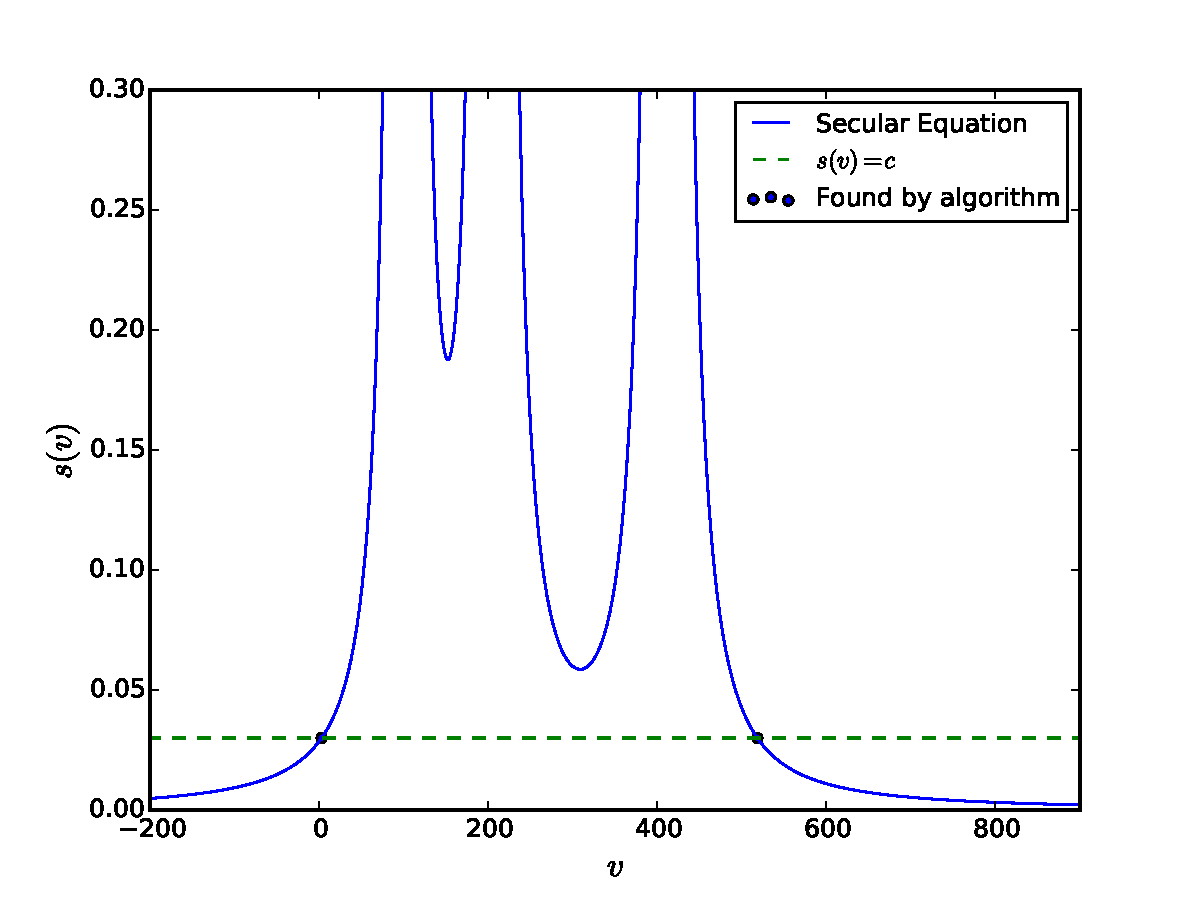
\includegraphics[width=0.7\linewidth]{images/secular}
%\caption{}
\label{fig:secular}
\end{figure}


The intersection of the curve and horizontal line is a graphical depiction of the "secular equation". To solve this equation, we need to find every intersection between the curve and horizontal line. There may be only two intersections, but there could be up to two for each diagonal element of $C$ (pole). It can be difficult to find all the intersections; each pole has between 0 and 2 solutions (we don't know how many beforehand), and poorly conditioned problems can strain even a carefully-designed solver.

Without additional information, we have no choice but to find every secular equation solution. We don't know which one solves $(P)$, so it appears we must check them all. But what if we knew that the leftmost solution would minimize the objective of $(P)$? Then we could solve a monotonically increasing function with exactly one root.

\section*{Statement}
Gander claims in \cite{gander1989} that the objective of $(P)$ is minimized when the smallest value of $\lambda$ is chosen. In other words, $(P)$ is equivalent to:


\begin{align*}
&(P') & \min~ & \lambda  \\
& s.t.& z^\top z &= s^2 \\
&& Cz &= \lambda z + b
\end{align*}


The proof of this claim is a trivial consequence of the following lemma.

\subsection*{Lemma}

If $(\lambda_1,z_1)$ and $(\lambda_2,z_2)$ solve \eqref{eq:first1} and \eqref{eq:first2}, and $\lambda_1 < \lambda_2$, then


\begin{align*}
z_1^\top C z_1 - 2b^\top z_1 &< z_2^\top C z_2 - 2b^\top z_2~.
\end{align*}


\subsection*{Proof}
We know that $(\lambda_1,z_1)$ and $(\lambda_2,z_2)$ solve \eqref{eq:first1}, so we have the following:

\begin{subequations}
\begin{align}
\label{eq:first3} Cz_1 &= \lambda_1 z_1 + b \\
\label{eq:first4} Cz_2 &= \lambda_2 z_2 + b
\end{align}
\end{subequations}


We can multiply both \eqref{eq:first3} and \eqref{eq:first4} by $z_1^\top$ and $z_2^\top$ to obtain:


\begin{subequations}
\begin{align}
\label{eq:2a}z_1^\top C z_1 &= \lambda_1 s^2 + z_1^\top b \\
\label{eq:2b}z_2^\top C z_2 &= \lambda_2 s^2 + z_2^\top b \\
\label{eq:2c}z_1^\top C z_2 &= \lambda_2z_1^\top z_2 + b^\top z_1 \\
\label{eq:2d}z_2^\top C z_1 &= \lambda_1z_2^\top z_1 + b^\top z_2 \end{align}
\end{subequations}


Note that I used \eqref{eq:first2} to replace instances of $z_1^\top z_1$ and $z_2^\top z_2$ by $s^2$. Now subtract \eqref{eq:2b} from \eqref{eq:2a} to obtain:


\begin{align*}
(z_1^\top C z_1 - z_1^\top b) - (z_2^\top C z_2 - z_2^\top b) &= (\lambda_1 - \lambda_2)s^2~.
\end{align*}


Add $b^\top z_2$ and subtract $b^\top z_1$ to yield:


\begin{align*}
O(z_1) - O(z_2) &= (\lambda_1 - \lambda_2)s^2 - z_1^\top b + z_2^\top b~,
\end{align*}


where $O(z)=z^\top C z - 2b^\top z$ is the objective value corresponding to $z$ in $(P)$. Now substitute \eqref{eq:2c} and \eqref{eq:2d}:


\begin{align*}
O(z_1) - O(z_2) &= (\lambda_1 - \lambda_2)s^2 + (\lambda_2 - \lambda_1) z_1^\top z_2 \\
&=  (\lambda_1 - \lambda_2)(s^2 - z_1^\top z_2)
\end{align*}


Note that $\lVert z_1 - z_2 \rVert = z_1^\top z_1 + z_2^\top z_2 - 2z_1^\top z_2 = 2s^2 - 2z_1^\top z_2$, so we have:


\begin{align*}
O(z_1) - O(z_2) &= \frac{1}{2}(\lambda_1 - \lambda_2)\lVert z_1 - z_2 \rVert
\end{align*}


Because $\lambda_1 < \lambda_2$, the right-hand size is negative. The objective value corresponding to $z_1$ is therefore less than that of $z_2$. Thus, solving $(P)$ means finding the smallest solution $\lambda$ that satisfies \eqref{eq:first1} and \eqref{eq:first2}; in other words, solving $(P)$ is equivalent to solving $(P')$.

This relationship between values of $\lambda$ in (P') and values of $O(z)$ in (P) is sufficient to prove our Theorem.

\bibliographystyle{IEEEtran}
% argument is your BibTeX string definitions and bibliography database(s)
\bibliography{bib}

\end{document}